\chapter{Accumulation of a Food Image Dataset}
\lhead{\emph{Accumulation of a Food Image Dataset}}

Before starting to experiment with machine learning algorithms for food classification, a dataset of food images needed to be created. In this chapter, reasons why the dataset is required are  explained and a process of accumulating the dataset is described.

\section{The Requirements for the Food Image Dataset}
 The dataset was needed because classification algorithms use the dataset to learn a classification model from it. The most important requirements to the dataset were:

\begin{enumerate}
  \item The images of the dataset should be taken under a real life conditions.
  \item There should be enough pictures in the dataset to learn a model for every machine learning algorithm that is going to be tried.
  \item Variance of food images of the same class should be high. 
\end{enumerate}

 
 It was critical, that food images taken in the lab conditions could not be used for training classification models. The intention of the project is to create the  models that could classify pictures of food taken by various users. People often use different angles and distance while taking pictures. The light conditions often vary greatly too. It is not possible to represent these variations under a lab environment. Therefore, it was crucial to use a food image dataset with high variance.

The dataset also needed to have many images that belong to each class. Having a lot of training samples is the best way to make sure that  the trained model is generalised and, thus, is able to  perform well on a test dataset. Simple models trained on a lot of data perform better than more elaborate models based on less data \citep{unreasonable}. Because of that, it was decided to have around  1,000 training images for each class in the dataset. 

Finally, an intra-class class variance of pictures in the training dataset should also be high. The problem of datasets with little variance can be illustrated with a dataset of tree images containing only pictures of trees with green leaves. The model learned by a classifier from this dataset will always classify a tree with orange leaves or a tree without leaves as a not tree. Therefore, a food dataset should also include a different kind of images for the same class, for example pizza with cheese, pepperoni pizza, and a slice of pizza. 

Accumulation of the dataset that satisfies these requirements was a challenging task. It would take a long time to take enough photos of meals for creating a big enough dataset. Also, a dataset containing images taken by only one or  few persons would not have enough variance. Because of that, possibilities to download food images from the Internet were explored.


It was observed that there are a lot of food images hosted on a photo sharing service flickr.com. Flickr has a Python API, that could be used to search for images according to their tags or titles, and  downloading them. Python script using this API was written. However, after downloading some images with a tag ``Fish and Chips",  it was realized that  a lot of downloaded images  contained this tag but were not actual food pictures e.g. \autoref{fig:fish}. Because of the time it would take to review every image, it was decided to try to find a publicly available food image dataset.  


\begin{figure}[ht]
\centering
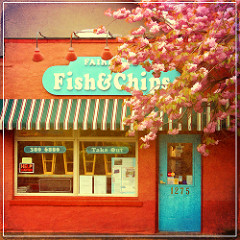
\includegraphics[width=2cm]{Figures/c3/flick.jpg}
\caption{Example of an Flickr Image with a Fish and Chips Tag}
\label{fig:fish}
\end{figure}


It was found that ImageNet Classification challenge, that was briefly described in \autoref{sec:intro}  includes many categories of food pictures. The only problem was that the number of images in different classes varies widely. Some classes like pizza has around 1300 pictures while other classes like salmon loaf has only 360 pictures. This problem was only discovered later when it was tried to train a classifier on this class. The classifier never picked salmon loaf class and was still able to achieve a high accuracy score. Therefore, it was chosen to use four categories of food which all have around 1300 pictures. These four classes were fish and chips, pizza, salad and vanilla ice-cream. 


Only four classes of images were selected because the dataset was required to be small enough to be trained on a laptop computer. Shorter algorithm training times are beneficial for exploring various configurations of algorithms.  It was considered that after investigating machine learning algorithms on four-class classification problem, it would be a relatively easy task to retrain the most accurate model using  a dataset containing either more classes of food images.

\section {Downloading the Dataset}
Since ImageNet publicly only provides links to the original hosts of image files,  a Python Script was written to read link from a text file, download the images from these links and save them to a disk.  The first problem that was faced after downloading the images, was that many pictures were either corrupted or were template images provided by hosting sites stating that the photo was no longer available. The script was modified to solve this problem by aborting the download and moving to a next image if a server returned a HTTP redirect. This code modification solved the problem of wrong images appearing in the downloaded dataset. However, the data set became much smaller than originally planned because many images that were no longer available were missing.  

To overcome this problem, a permission to access the original ImageNet download files was requested. The permission was granted after agreeing to use the dataset only for non-commercial research and educational purposes. It allowed accessing the original data set with all images included. The original archives were downloaded using a python script and then extracted.

\section {Creating the  Dataset}
Python class named Data was created to handle a creation of the image dataset. The class was designed to allow images to be loaded using various methods. The constructor of the class takes one argument: the relative path to the folder, where the data is located. Images can be loaded from a pickle file located in /pickle folder, extracted from .tar archives, or can be read directly from a /images folder. Loading the files from  a pickle is the fastest method because Python only needs to read one file compared to thousands of files while loading  separate images. To allow saving dataset to a pickle file,  a Python method was created. A pickle is a binary file representing a Python object. The pickle file was structured as a list of classes of every picture, followed by a list of actual images. Method try\_download\_images was used to download the  datasets from the  ImageNet. This method takes two arguments - a username and the ImageNet access key. The extract method   was  used to extract downloaded .tar archive files into the pictures folder. Method resize\_image was  written to  make  resizing  images in the dataset easier. It takes a list with height and width of requested image size and resizes the images.  Finally, train\_test\_split method was writen. It can be used to shuffle the data and split it into training and testing datasets. It takes an optional argument- a fraction that shows a percentage of data to be used for testing the classifier. These methods for manipulating datasets will be later used to preprocess data for the classification.

\section{Summary}
In this chapter, the requirements for the dataset were defined. The most important rule for the image dataset was to have many pictures of each class  taken under real life conditions. To fulfill this requirement, it was decided to download food images from the ImageNet. It was decided to use four food classes, to reducing the complexity. Finally, the class for preprocessing and manipulating the dataset was created.  In the following chapter, machine learning algorithms are introduced and classifiers uaing these algorithms are built.